\documentclass[preprint,notoc]{JHEP3}
\usepackage{epsfig}

\def\Vind{V^{\rm induced}}
\def\eslt{\not\!\!{E_T}}
\def\eslt{E_T^{\rm miss}}
\def\emiss{\not\!\!{E}}
\def\to{\rightarrow}
\def\Phat{\hat{\Phi}}
\def\bi{\begin{equation}gin{itemize}}
\def\ei{\end{itemize}}
\def\te{\tilde e}
\def\c1p{C1^\prime}
\def\ta{\tilde a}
\def\tG{\widetilde G}
\def\th{\tilde h}
\def\tH{\tilde H}
\def\tl{\tilde l}
\def\tu{\tilde u}
\def\tc{\tilde c}
\def\ta{\tilde a}
\def\ts{\tilde s}
\def\tb{\tilde b}
\def\tf{\tilde f}
\def\td{\tilde d}
\def\tQ{\tilde Q}
\def\tL{\tilde L}
\def\tH{\tilde H}
\def\tst{\tilde t}
\def\ttau{\tilde \tau}
\def\tmu{\tilde \mu}
\def\tg{\tilde g}
\def\tnu{\tilde\nu}
\def\tell{\tilde\ell}
\def\tq{\tilde q}
\def\tB{\widetilde B}
\def\tw{\widetilde W}
\def\tz{\widetilde Z}
\def\mgut{M_{\rm GUT}}
%\def\tw{\tilde\chi}
%\def\twp{\tilde\chi^+}
%\def\twm{\tilde\chi^-}
%\def\twpm{\tilde\chi^\pm}
%\def\tz{\tilde\chi^0}
%\def\alt{\stackrel{<}{\sim}}
%\def\agt{\stackrel{>}{\sim}}
\def\alt{\lesssim}
\def\agt{\gtrsim}
%\def\begin{equation}{\begin{equation}gin{equation}}  
%\def\end{equation}{\end{equation}}  
%\def\begin{eqnarray}{\begin{eqnarray}}  
%\def\end{eqnarray}{\end{eqnarray}}  
\def\CM{\cal M}
\def\sigv{\langle \sigma v \rangle}
\def\To{\Rightarrow}
\def\to{\rightarrow}
\newcommand\drv[2]{\frac{\partial #1}{\partial #2}}
\newcommand\Drv[2]{\frac{d #1}{d #2}}
\def\tb{{\tilde{b}}}
\def\dm{{\chi}}

\title{Validation - Conversion Driven Freeze-Out}
\author{Andre Lessa}
\abstract{}


\begin{document}

\section{General Boltzmann Equations}

Below we summarize the set of coupled Boltzmann equations and the definitions of the terms
entering each of them:

\begin{itemize}
\item Entropy:
\begin{equation}
\frac{d N_S}{d x} = \frac{e^{(3 x - N_S)}}{HT} \sum_{i} BR(i,X) \Gamma_i m_i \left(n_i -
\mathcal{N}_{i}^{th} \right) \label{eq:Sfin}
\end{equation}
\item Number densities:
\begin{eqnarray}
\frac{d N_i}{d x} & = & -3
+ \frac{n_i}{H}\left( \frac{\bar{n}_i^2}{n_i^2} -1 \right) \langle \sigma v \rangle_{ii} 
+ \frac{1}{H} \sum_{j\neq i} \left( \frac{\bar{n}_i}{n_i} \bar{n}_j - n_j \right) \langle \sigma v \rangle_{ij}
+ \frac{n_i}{H} \sum_{j\neq i} \left(\frac{\bar{n}_i^2}{n_i^2}\frac{n_j^2}{\bar{n}_j^2}  - 1 \right) \langle \sigma v \rangle_{jj} \nonumber\\
&+& \frac{1}{H} \sum_{j\neq i} \left(\frac{\bar{n}_i}{n_i}\frac{n_j}{\bar{n}_j}  - 1\right)  \tilde{\Gamma}_{ijSM} 
 -  \frac{\Gamma_i}{H} \frac{m_i}{R_i}\left(1 - \frac{\mathcal{N}_{i}^{th}}{n_i} \right)
  +  \sum_{j \neq i} \mathcal{B}_{ji}^{eff} \frac{\Gamma_j}{H}
 \frac{m_j}{R_j}\left(\frac{n_j}{n_i} - \frac{\mathcal{N}_{ji}^{th}}{n_i}  \right)
\end{eqnarray}
\item Energy density ratios:
\begin{equation}
\frac{ d R_i}{d x} =   -3 \frac{P_i}{n_i} + \sum_{j \neq i} \mathcal{B}_{ji}^{eff}
\frac{\Gamma_j}{H} m_j \left( e_{inj}^{ji} - \frac{R_i}{R_j} \right) \left(\frac{n_j}{n_i} -
\frac{\mathcal{N}_{ji}^{th}}{n_i} \right)
\end{equation}
\end{itemize}
where:
\begin{eqnarray*}
x & = & \ln(R/R_0) \mbox{, } N_S = \ln(S/S_0) \mbox{, } N_i = \ln(n_i/n_i^0) \mbox{ and } R_i = \frac{\rho_i}{n_i} \mbox{ (variables)}\\
\langle \sigma v \rangle_{ii} & =  &\frac{1}{\bar{n}_i^2}\int  d\Pi_{i} d\Pi_{j} d\Pi_{a} d\Pi_{b} (2 \pi)^4 \delta^{(4)}(P) |M|^2 e^{-(E_i + E_j)/T}  \mbox{ (self-annihilation to SM)}\\
\langle \sigma v \rangle_{ij} & = & \frac{1}{\bar{n}_i \bar{n}_j}\int  d\Pi_{i} d\Pi_{j} d\Pi_{a} d\Pi_{b} (2 \pi)^4 \delta^{(4)}(P) |M|^2 e^{-(E_i + E_j)/T}  \mbox{ (co-annihilation)} \\
\langle \sigma v  \rangle_{jj} & =  &\frac{1}{\bar{n}_i^2}\int  d\Pi_{i} d\Pi_{j} d\Pi_{a} d\Pi_{b} (2 \pi)^4 \delta^{(4)}(P) |M|^2 e^{-(E_i + E_j)/T}   \mbox{ (self-annihilation to BSM)}\\
\tilde{\Gamma}_{ijSM} & =  &\frac{1}{\bar{n}_i}\int  d\Pi_{i} d\Pi_{j} d\Pi_{a} d\Pi_{b} (2 \pi)^4 \delta^{(4)}(P) |M|^2 e^{-(E_i + E_j)/T}    \mbox{ (conversion rate)}\\
\mathcal{N}^{th}_{i} & = &  \bar{n}_i \sum_{i \to \ldots} BR(i \to 1 + 2 +
\ldots) \prod_{k=1,2,..} \frac{n_k}{\bar{n}_k} \mbox{ (effective decay density)}\\
\mathcal{N}^{th}_{ji} & = & \frac{\bar{n}_j}{\mathcal{B}^{eff}_{ji}}
\sum_{j \to i + \ldots} g_Y BR(j \to g_i i + 1 + \ldots) \left(\frac{n_i}{\bar{n}_i}\right)^{g_i} \prod_{k=1,..} \frac{n_k}{\bar{n}_k} \mbox{ (effective injection density)}\\
\mathcal{B}^{eff}_{ji} & = & \sum_{j \to i + \ldots} g_i BR(j \to g_i i +
1+\ldots) \mbox{ (effective branching ratio)}\\
e_{inj}^{ji} & = &  \frac{1}{2}\left(1+\frac{m_i^2}{m_j^2}\right)  \mbox{ (effective energy injection)}\\
BR(i,X) & = & \frac{E_{\gamma}}{E_i} \mbox { (effective energy injected in the thermal bath)} 
\end{eqnarray*}

Finally,  we can approximate the $P_i/n_i$ function for all values of $R_i$ by:
\begin{equation}
\frac{P_i}{n_i} = \left\{ \begin{array}{rl}
& \frac{2 m_i}{3}\left( \frac{R_i}{m_i} -1 \right) + m_i \sum_{n >1} a_n \left(\frac{R_i}{m_i} -1 \right)^n  \mbox{ , for $R_i < \tilde{R}$} \\
& \frac{R_i}{3}  \mbox{ , for $R_i > \tilde{R}$} 
\end{array} \right. \label{Pfin}
\end{equation}
where the coefficients $a_n$ are given by the numerical fit and $\tilde{R}$ is given by the matching of the two solutions.


\section{Simplified Model}

The simplified model considered here corresponds to the SM added by a sbottom-like mediator ($\tb$) and a bino-like dark matter particle ($\dm$). The relevant lagrangian is:

\begin{equation}
\mathcal{L}_{int} = |\mathcal{D}_\mu \tb|^2 + \lambda_{\dm} \tb \bar{b} \frac{1-\gamma_5}{2} \dm + h.c.
\end{equation}

Furthermore the masses are assumed to be: $m_\tb = 510$~GeV, $m_\dm = 500$~GeV.
In this case the thermal cross-section $\langle \sigma v  \rangle_{\tb \tb}$ and the conversion rates $\tilde{\Gamma}_{\tb \dm SM}$, $\tilde{\Gamma}_{\dm \tb SM}$are shown in Fig.\ref{fig:rates}.

\begin{figure}[h]
	\centering
	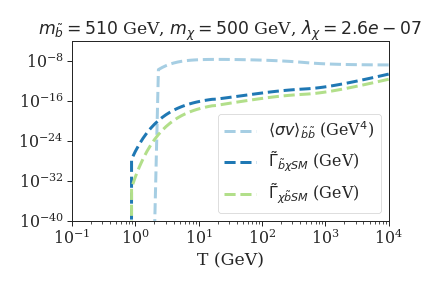
\includegraphics[scale=0.7]{rates.png}
	\caption{The mediator annihilation rate and the conversion rate for $\tb + SM \to \dm + SM$
	and $\dm + SM \to \tb + SM$ as function of temperature.} \label{fig:rates}
\end{figure}

\section{Examples}

\subsection{Simple Freeze-out}

In this scenario we assume no conversion rate and   $\langle \sigma v  \rangle_{\dm \dm} = \langle \sigma v  \rangle_{\tb \tb} \equiv \langle \sigma v \rangle$, where the latter is the curve shown in Fig.\ref{fig:rates}.
We also take the conversion rates ( $\tilde{\Gamma}_{ij SM}$) to be zero and the $\tb$ width
to be small, so it decays after freeze-out. Finally, in this simplified scenario, we assume that the 
entropy injection is negligible ($BR(\tb,X) = 0$), so we have:

\begin{eqnarray*}
\frac{d N_S}{d x} & = & 0\\
\frac{d N_\dm}{d x} & = & -3
+ \frac{n_\dm}{H}\left( \frac{\bar{n}_{\dm}^2}{n_{\dm}^2} -1 \right) \langle \sigma v \rangle 
+  \frac{\Gamma_\tb}{H} \frac{m_\tb}{R_\tb} \left(\frac{n_\tb}{n_\dm} - \frac{\bar{n}_\tb}{\bar{n}_\dm}  \right) \\
\frac{d N_\tb}{d x} & = & -3
+ \frac{n_\tb}{H}\left( \frac{\bar{n}_{\tb}^2}{n_{\tb}^2} -1 \right) \langle \sigma v \rangle 
-  \frac{\Gamma_\tb}{H} \frac{m_\tb}{R_\tb} \left( 1 - \frac{\bar{n}_\tb n_\dm}{n_\tb \bar{n}_\dm}  \right)\\
\frac{ d R_\dm}{d x} & = &   -3 \frac{P_\dm}{n_\dm} +  \frac{\Gamma_\tb}{H} m_\tb \left( \frac{1}{2} + \frac{m_\dm^2}{2 m_\tb^2}- \frac{R_\dm}{R_\tb} \right) \left(\frac{n_\tb}{n_\dm} - \frac{\bar{n}_\tb}{\bar{n}_\dm}  \right) \\
\frac{ d R_\tb}{d x} & = &   -3 \frac{P_\tb}{n_\tb}
\end{eqnarray*}




\end{document}